\chapter{Pomiary wibrometrem skanującym}
\label{cha:Measurments}

W celu przetestowania powstałego urządzenia przeprowadzono pomiary wibracji blachy pod wpływem szumu białego. Celem pomiarów było stworzenie map w kolejnych tercjach. Każda mapa składała się z zestawu punktów, gdzie każdy punkt przedstawiał prędkość drgań blachy w danym punkcie pomiarowym.

\section{Stanowisko Pomiarowe}
Szum został wygenerowany przy pomocy generatora Bruel\&Kjaer 1405, wzmacniacza oraz głośnika znajdującego się w komorze pogłosowej Laboratorium Akustyki Technicznej. Natomiast, jako że wyjściem wibrometru jest sygnał ciągły dźwiękowy, do zebrania próbek sygnału użyto karty dźwiękowej. W celu zebrania pomiarów powstał skrypt w języku Matlab, który wchodził w interakcję zarówno z kartą dźwiękową, w celu zapisywania próbek dźwięku, oraz z systemem pozycjonowania powstałym w ramach tej pracy, w celu przemieszczania wibrometru. Opisywane stanowisko przedstawione jest na zdjęciu \ref{img:meas_setup}.

\begin{figure}[h!] 
\centering 
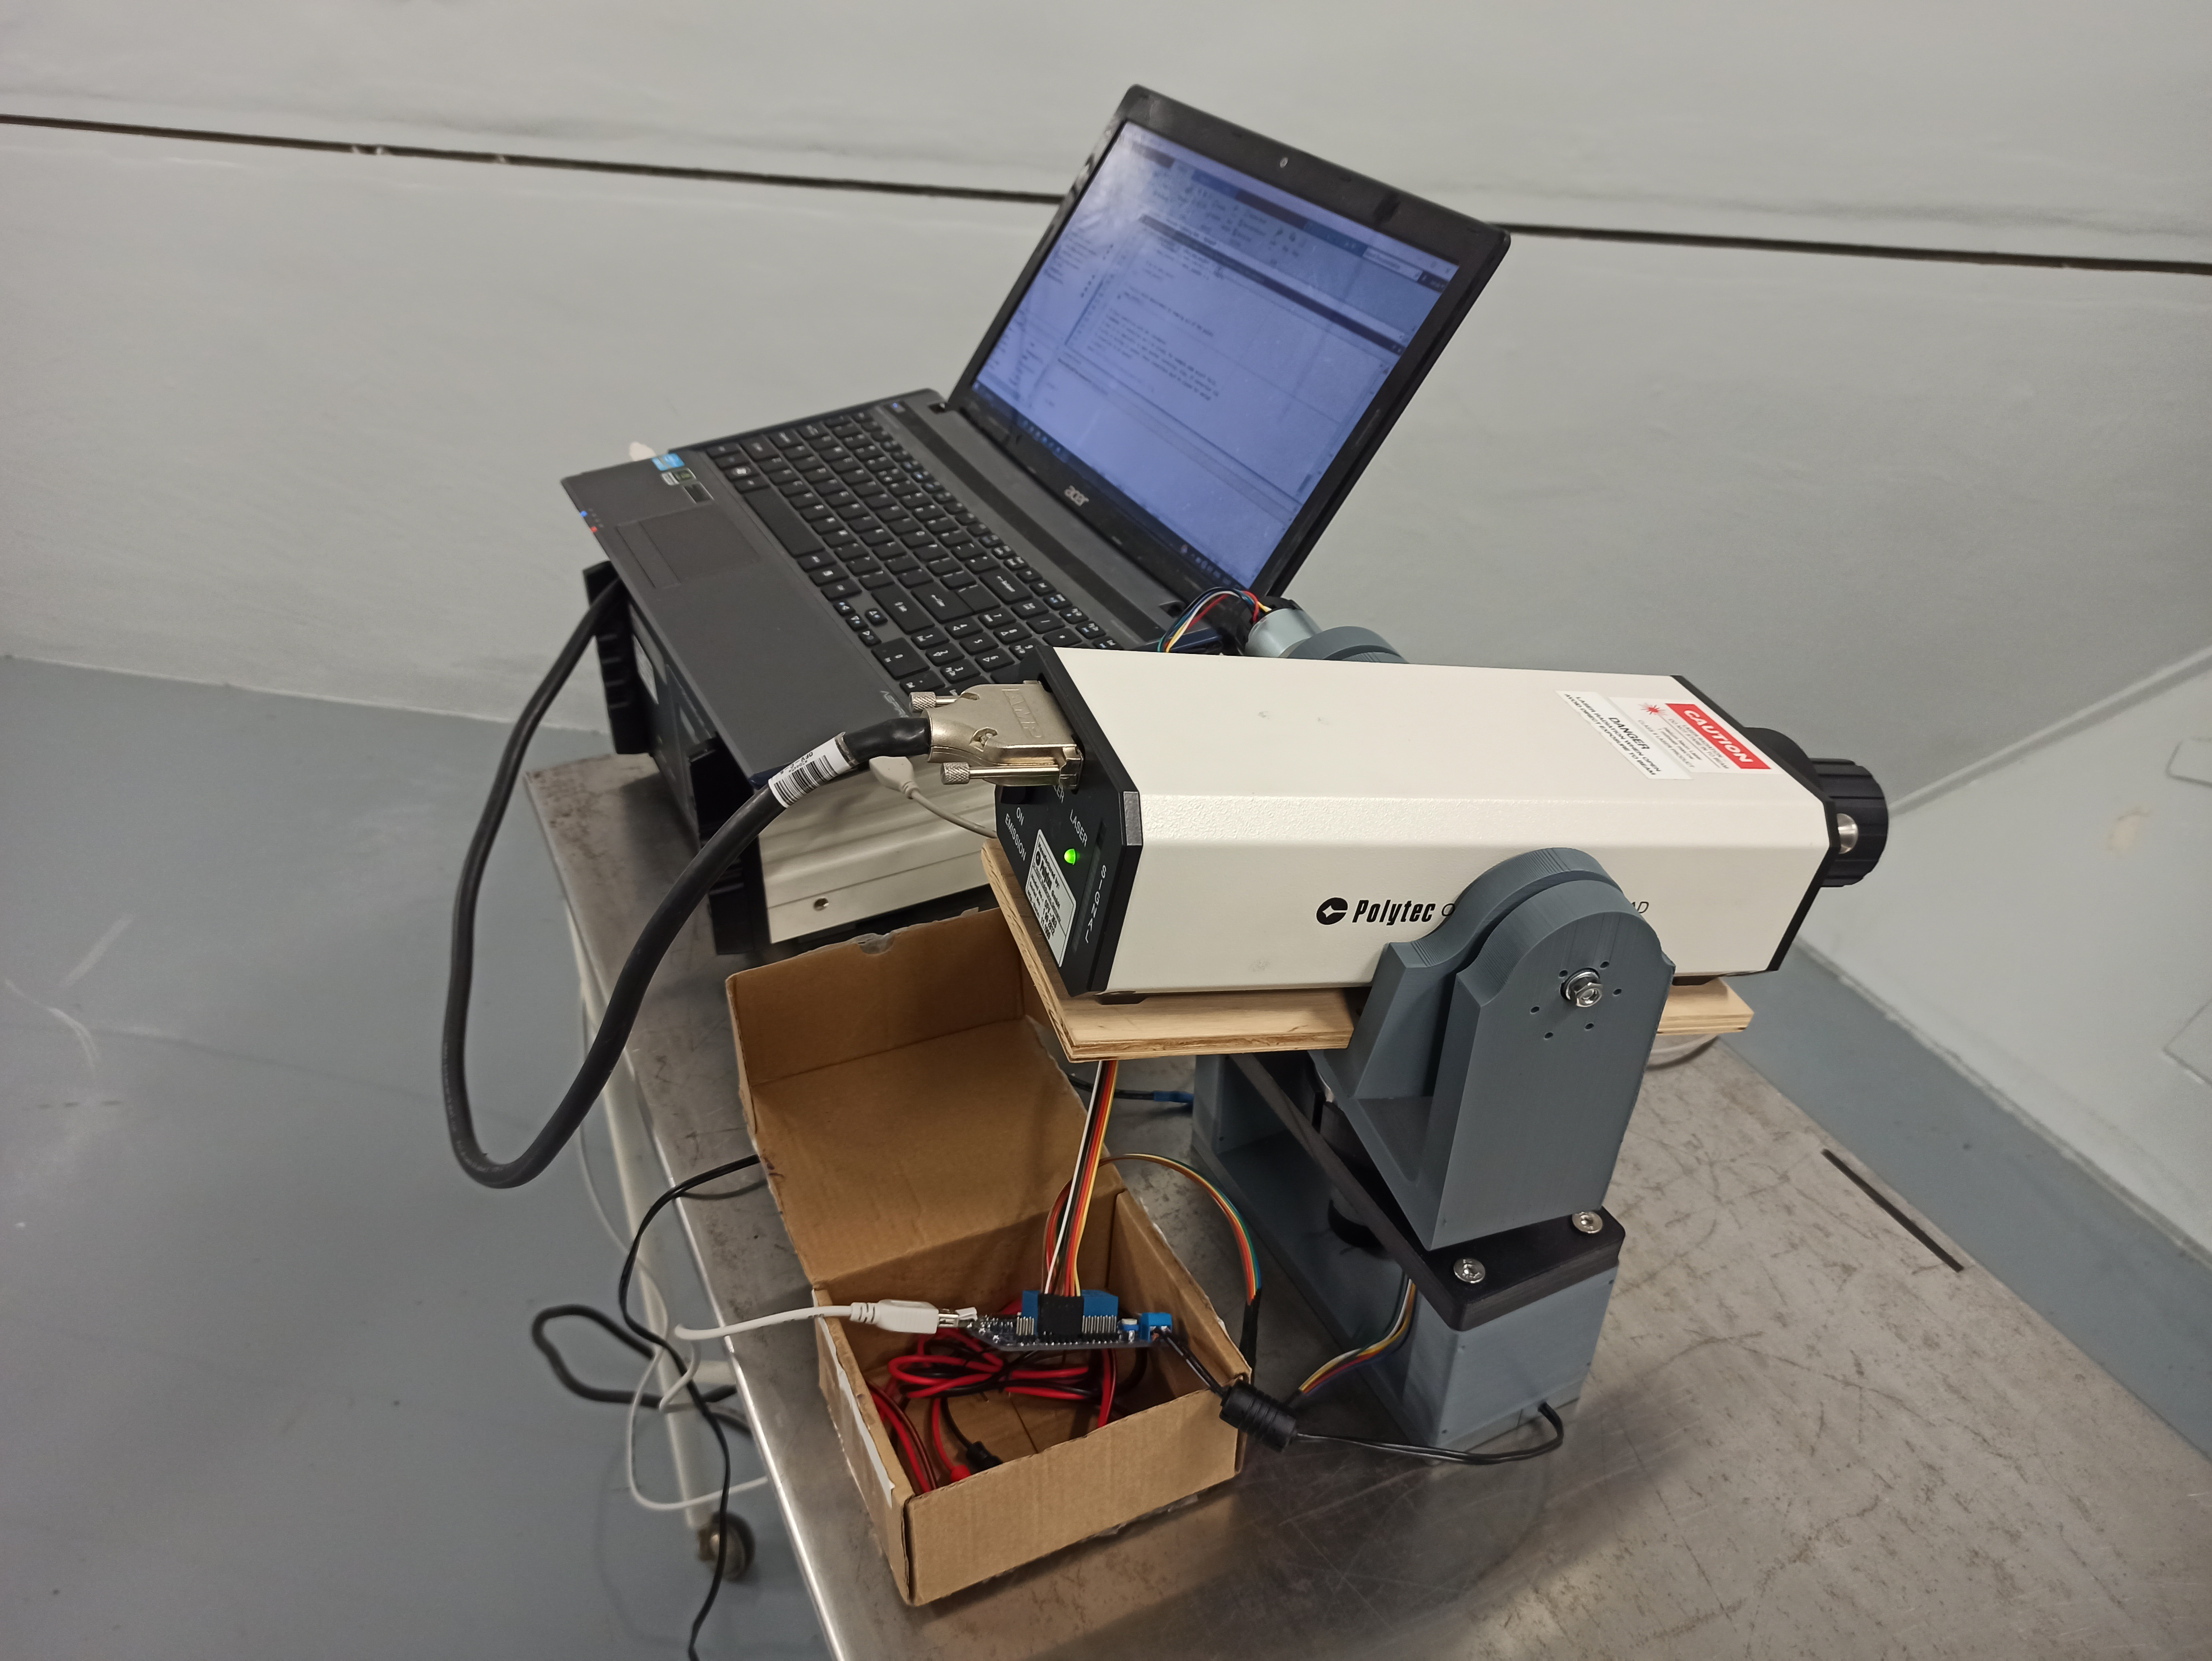
\includegraphics[width=0.6\textwidth]{img/MeasSetup.jpg}
\caption{Stanowisko pomiarowe.}
\label{img:meas_setup}
\end{figure}

\section{Algorytm zbierający dane}
Z kąta ustawienia metalowej płyty względem ziemi, odległości ustawienia wibrometru względem płyty, oraz zakresów ruchu wibrometru, wynikał zakres w jakim została płyta przeskanowana. Obrót dookoła osi yaw, czyli z, został ustawiony na zakres $\pm9^{\circ}$, co w odległości, w jakiej został ustawiony wibrometr, daje pełną szerokość płyty, czyli $40 cm$. Bardziej problematyczna była oś pitch, czyli obrót dookoła osi y. Ponieważ mierzona płyta była ustawiona pod kątem $50^{\circ}$ do podłoża, a wibrometr był w stanie zniżyć się maksymalnie o $30^{\circ}$. Oznaczało to, że pozycja w której wibrometr jest ustawiony poziomo jest odchylona od płaszczyzny pomiarowej o $40^{\circ}$. Dlatego też zdecydowano się na ustawienie zera relatywnego dla tej osi na kącie $20^{\circ}$, ponieważ wtedy laser celował w górę płyty, a zakres ruchu wibrometru ustalono na $0^{\circ}$-$10^{\circ}$, czyli o jeden stopień ponad połowę płyty. Natomiast na potrzeby późniejszych obliczeń zapisano wartość $-20^{\circ}$ jako przesunięcie pozycji zero tej osi wibrometru względem faktycznej osi prostopadłej do powierzchni blachy. Dokładny schemat przedstawiający ułożenie wibrometru w osi pitch znajduje się na rys \ref{img:pitch_schematic_drawing}. W tym miejscu można także zaznaczyć, że z punktu widzenia końcowego pomiaru nie ma znaczenia, czy jako oś zero zostanie ustalona faktyczna oś pozioma i późniejsze przesunięcie będzie wynosić $-40^{\circ}$ zamiast $-20^{\circ}$, czy zostanie to zrobione tak jak w przypadku tego pomiaru - oś zerowa zostanie przesunięta względem osi poziomej. Jest to wybór, który pozostaje w gestii osoby dokonującej pomiarów. Ważnym jest aby być świadomym kątów, pod jakimi zostały zbierane pomiary w celu późniejszej analizy danych.

\begin{figure}[h!] 
\centering 
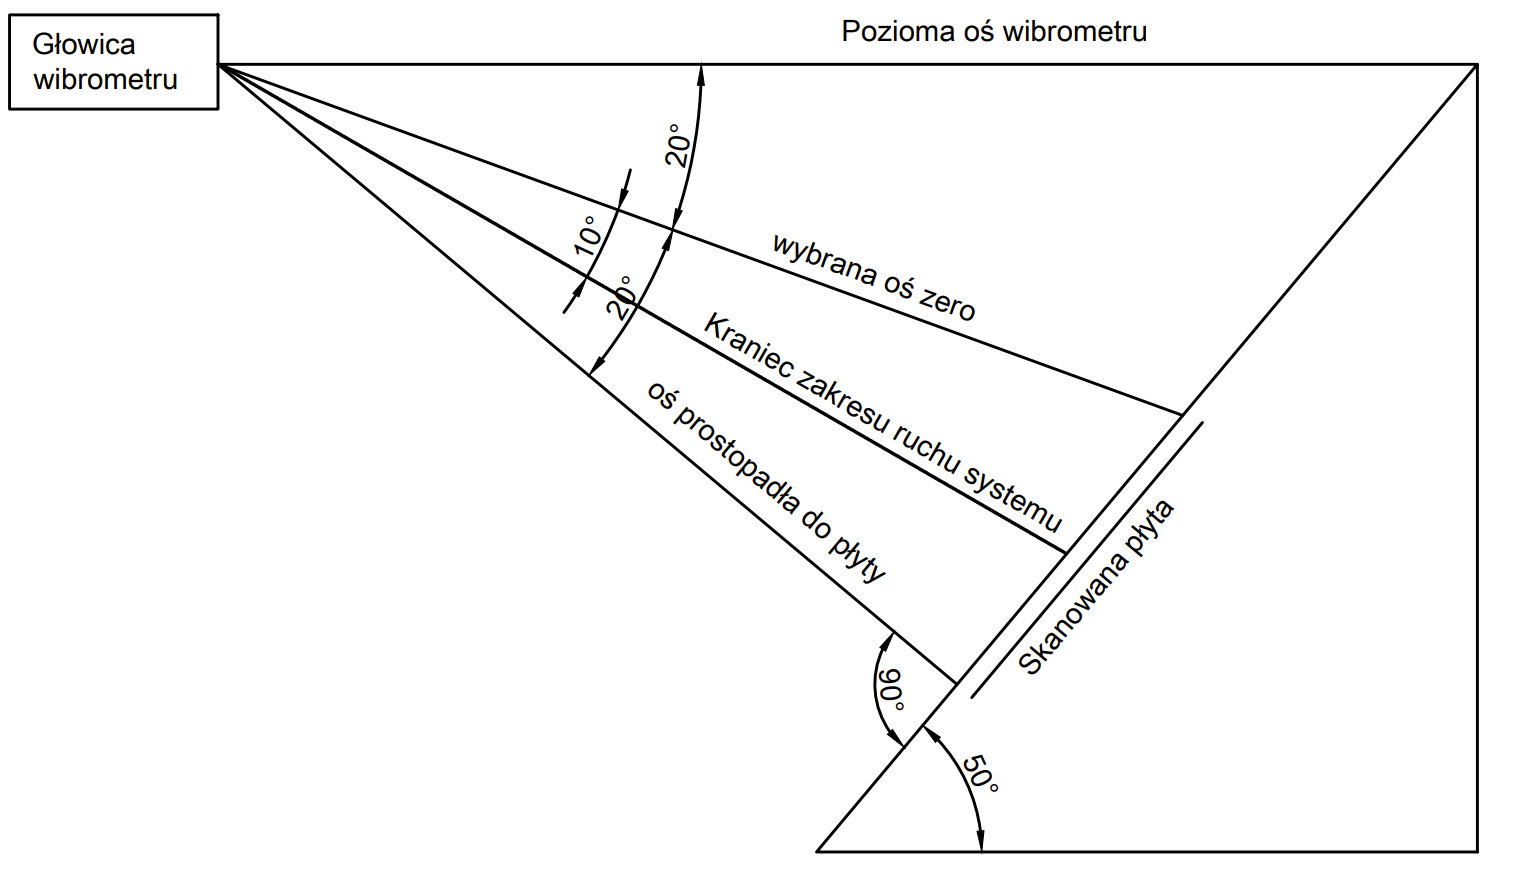
\includegraphics[width=\textwidth]{img/pitch_meas_schematic_draw.png}
\caption{Schemat ustawienia wibrometru w osi pitch.}
\label{img:pitch_schematic_drawing}
\end{figure}

Po inicjalizacji systemu, która jako argumenty przyjmuje właśnie powyższe wartości kątów, następuje pomiar w pętli, która trwa, dopóki system nie przejdzie w status Finished, kiedy to wykonywany jest ostatni pomiar oraz dane zapisywane są do pliku .mat. W każdym punkcie pomiarowym skrypt odczekuje $2s$, aby ustabilizować drgania wibrometru wynikające z plastikowej (drukowane w 3D) konstrukcji, oraz zbiera pięcio-sekundową ($5s$) próbkę dźwięku (używając metody \texttt{recordblocking()} z klasy \texttt{audiorecorder}), z częstotliwością próbkowania $8kHz$. Dodatkowo zapisywana jest dokładna pozycja wibrometru (używając metody \texttt{get\_point()} z klasy \texttt{VibrometerAPI}). Wszystkie te informacje zmierzone w punkcie zapisywane są do listy struktur, która to po skończonych pomiarach zapisywana jest do pliku .mat. Dokładny algorytm przedstawiony jest na schemacie \ref{img:matlab_data_acq_uml}.

\begin{figure}[h!] 
\centering 
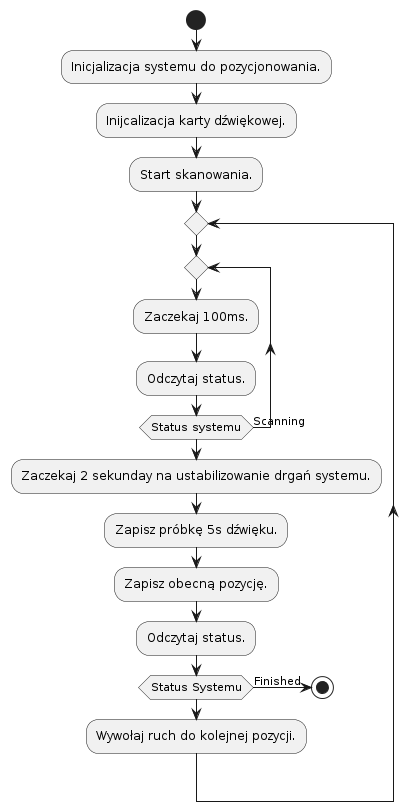
\includegraphics[width=0.7\textwidth]{img/MatlabDataAcq.png}
\caption{Uproszczony algorytm zbierający danych.}
\label{img:matlab_data_acq_uml}
\end{figure}



\section{Algorytm analizujący dane}
Algorytm analizujący dane jako swoje wejście wczytuje plik, zawierający  listę struktur ze wszystkimi zmierzonymi punktami, natomiast jego wyjściem jest zestaw wykresów, po jednym dla każdego analizowanego pasma częstotliwości.

\begin{figure}[h!] 
\centering 
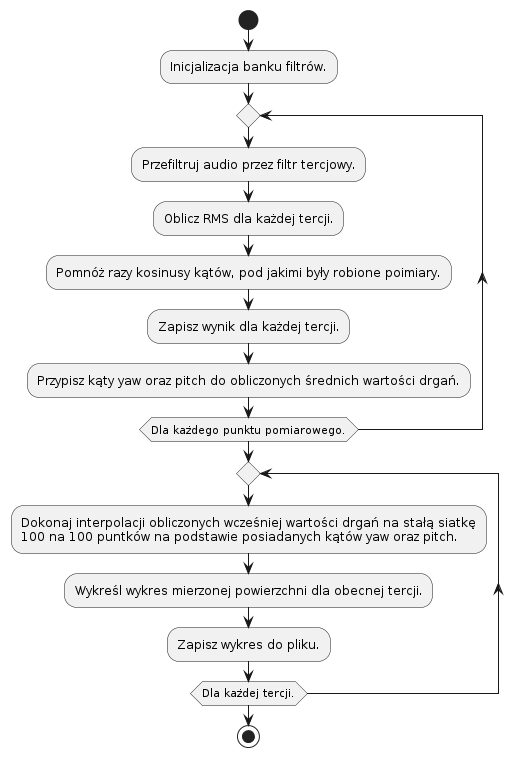
\includegraphics[width=0.7\textwidth]{img/AnalyseDataUML.png}
\caption{Algorytm analizy danych pomiarowych.}
\label{img:analyse_data_uml}
\end{figure}

Pierwszy krok algorytmu to iteracja po wszystkich odwiedzonych przez wibrometr punktach. W każdym punkcie należy rozbić sygnał na częstotliwości, w tym przypadku na tercje w zakresie $22Hz$ do $4kHz$, za pomocą filtru z klasy \texttt{octaveFilterBank}. W tym zakresie wspomniany filtr stworzył 26 tercji. Następnie, nadal w pętli po punktach, dla każdej z tych tercji, należy policzyć średnią za pomocą funkcji \texttt{rms}. Daje to średnią prędkość drgań danego punktu w danym zakresie częstotliwości. Kolejnym krokiem jest uwzględnienie faktu, że pomiar odbywał się pod kątem do powierzchni. Aby tego dokonać, obliczoną średnią energię należy pomnożyć razy cosinus kąta, pod jakim został dokonany pomiar, zarówno dla osi obrotu pitch jak i yaw. Należy także pamiętać o przesunięciu, czyli uwzględnieniu $-20^{\circ}$ dla osi pitch. Po wyjściu z pętli w odpowiednich zmiennych znajdują się informacje o średniej energii drgań we wszystkich tercjach oraz we wszystkich punktach. Dodatkowo, nadal istotna jest znajomość koordynatów tych punktów, aby poprawnie je zaznaczyć na wykresie. Ostatnim krokiem algorytmu jest pętla iterująca po 26 tercjach - dla każdej tercji należy przeprowadzić interpolację punktów oraz nakreślić je na wykresie. Dokładny algorytm znajduje się na schemacie \ref{img:analyse_data_uml}.



\section{Wyniki pomiarów}
W pierwszej kolejności zmierzono w kilku losowych punktach wartości drgań tła, czyli drgania bez włączonego głośnika. Przykładowo, wykres \ref{img:background_noise_graph} przedstawia drgania szumu w punkcie startowym równym $yaw = 0$ oraz $pitch = 0$. Wykres pokazuje, że w dolnych zakresach częstotliwości, wartości drgań są na poziomie części tysięcznych ($2 \cdot 10 ^ {-3}$), a w wyższych częstotliwościach schodzą nawet do części dziesięciotysięcznych ($5 \cdot 10 ^ {-4}$). W dalszych pomiarach wartości te będą stanowiły referencję, określającą czy wibrometr zbiera faktyczną wiązkę odbitą, czy zaledwie szumy tła.

\begin{figure}[h!] 
\centering 
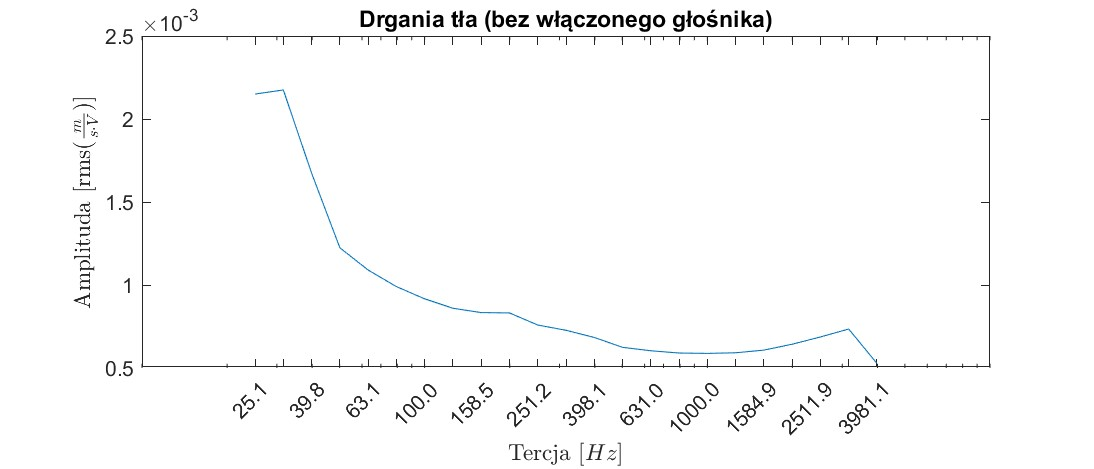
\includegraphics[width=\textwidth]{img/BackgroundGraph.jpg}
\caption{Szum drgań tła.}
\label{img:background_noise_graph}
\end{figure}

W drugiej kolejności wykonano opisywany wcześniej właściwy pomiar. Najmocniejsze drgania zarejestrowano dla tercji $31.6Hz$, ponieważ sięgały aż $0.22 \frac{m}{s \cdot V}$ na środku płyty, a $0.02 \frac{m}{s \cdot V}$ na rogach płyty. Jest to aż kolejno $100$ krotnie (dla środka płyty) oraz $10$ krotnie (dla brzegów płyty) więcej, niż zmierzone wcześniej tło. Rozkład drgań dla tercji $31.6Hz$ przedstawia wykres \ref{img:2_GraphThird}.

\begin{figure}[h!] 
\centering 
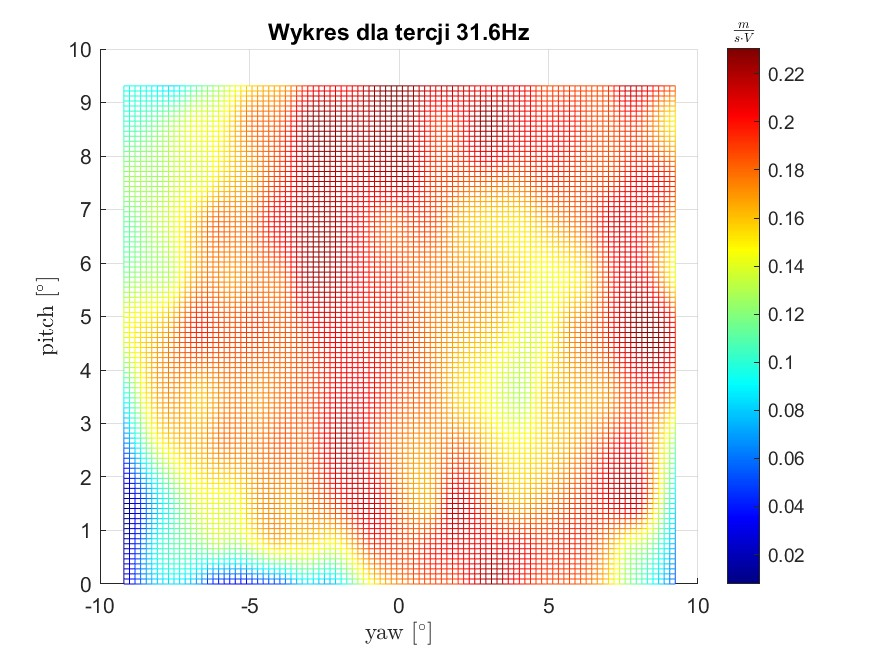
\includegraphics[width=0.8\textwidth]{img/2_GraphThird.jpg}
\caption{Rozkład drgań dla tercji $31.6Hz$.}
\label{img:2_GraphThird}
\end{figure}

Dla trzech pierwszych tercji, o częstotliwościach środkowych $25.1Hz$, $31.6Hz$, $39.8Hz$ nie widać żadnych wyraźnie zaznaczonych mod drgań. Natomiast w tercji o częstotliwości środkowej $50.1Hz$, widać wyraźnie zaznaczoną modę znajdującą się w lewej połówce badanej płyty. Wykres drgań płyty dla tej tercji przedstawia rysunek \ref{img:4_GraphThird}. Pokazuje on opisywany wyraźny wzrost prędkości drgań w lewej połówce płyty, blisko krawędzi. Porównując ten wykres z pozostałymi można także zauważyć ciekawe zjawisko. Płyta w tej częstotliwości drga dosyć intensywnie blisko krawędzi, pomimo że była ona przy krawędziach przytwierdzona do podłoża. Jest to także jedyna tercja, gdzie płyta drga intensywniej po lewej stronie, niż po prawej stronie. Natomiast biorąc pod uwagę, że pasta którą przytwierdzono płytę do podłoża nie była równomiernie rozłożona, oraz płyta nie była idealnie wypolerowana, zjawiska takie są oczekiwane.

\begin{figure}[h!] 
\centering 
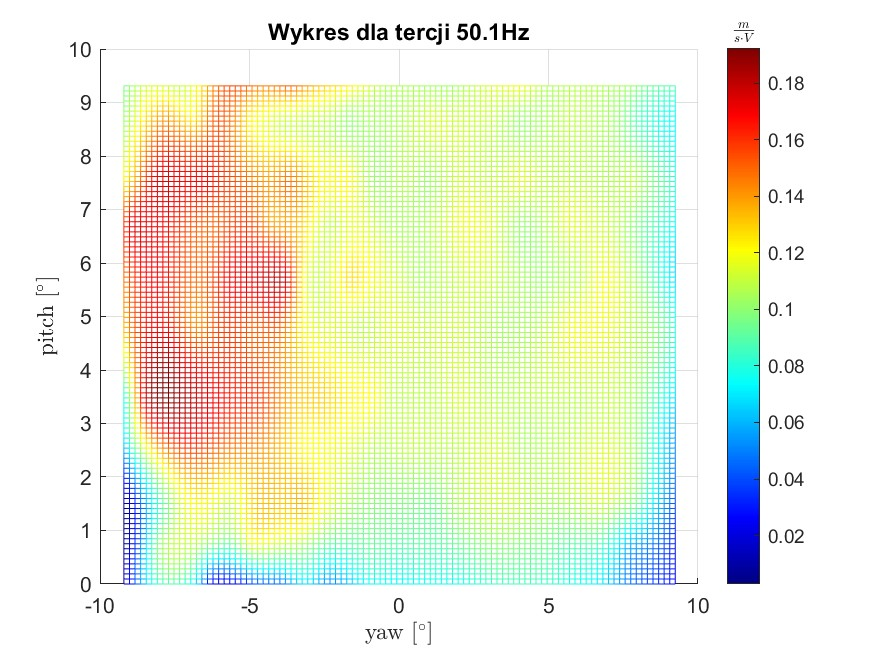
\includegraphics[width=0.8\textwidth]{img/4_GraphThird.jpg}
\caption{Rozkład drgań dla tercji $50.1Hz$.}
\label{img:4_GraphThird}
\end{figure}

Tak jak już wspomniano powyżej, tercja o częstotliwości środkowej $50.1Hz$ jest jedyna, gdzie drgania są wyraźniejsze po lewej stronie płyty. Już dla kolejnej tercji, o częstotliwości $63.1Hz$, widać wyraźne przesunięcie strzałki fali w prawą połówkę płyty. Rozkład drgań dla tercji $63.1Hz$ przedstawiony jest na wykresie \ref{img:5_GraphThird}. Podobne zachowania można zaobserwować także dla dwóch kolejnych tercji o częstotliwościach $79.4Hz$ oraz $100Hz$.

\begin{figure}[h!] 
\centering 
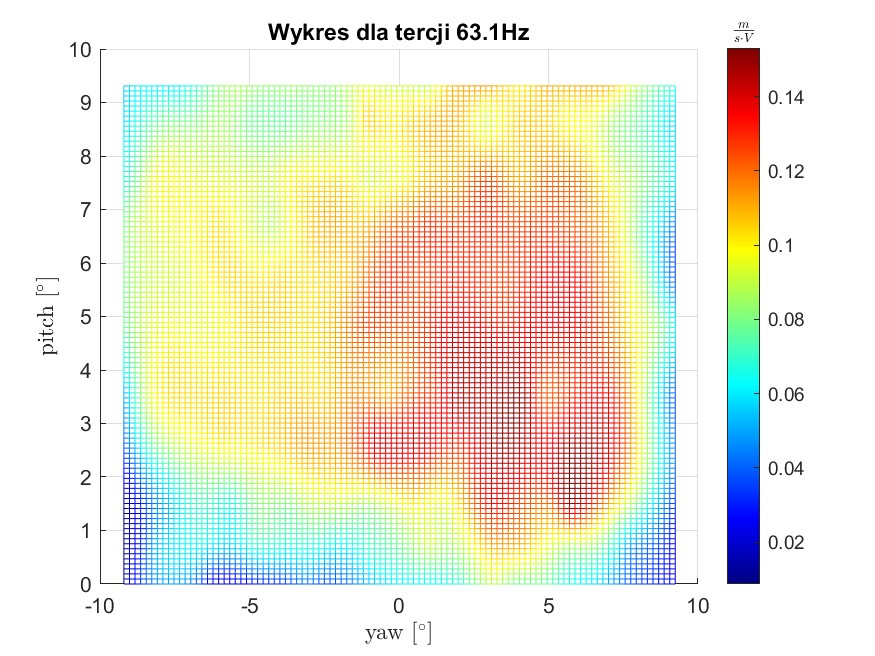
\includegraphics[width=0.8\textwidth]{img/5_GraphThird.jpg}
\caption{Rozkład drgań dla tercji $63.1Hz$.}
\label{img:5_GraphThird}
\end{figure}

Tak samo jak dla samego tła, amplituda drgań w wyższych częstotliwościach zaczyna zanikać dość gwałtownie. Przykładowo, dla tercji $125.9Hz$ widać wyraźny zanik drgań. Wysoka amplituda zachowała się jedynie w dwóch punktach. Rozkład drgań dla tej tercji przedstawia wykres \ref{img:8_GraphThird}. Natomiast już w kolejnej tercji, $158.5Hz$, także i te dwa punkty zanikają, co przedstawia wykres \ref{img:9_GraphThird}.

\begin{figure}[h!] 
\centering 
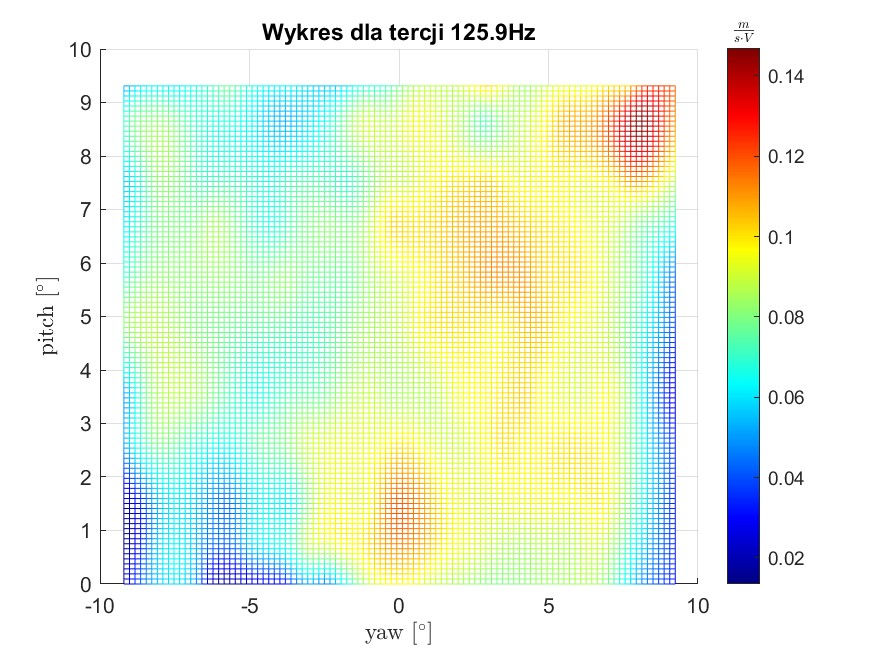
\includegraphics[width=0.8\textwidth]{img/8_GraphThird.jpg}
\caption{Rozkład drgań dla tercji $125.9Hz$.}
\label{img:8_GraphThird}
\end{figure}

\begin{figure}[h!] 
\centering 
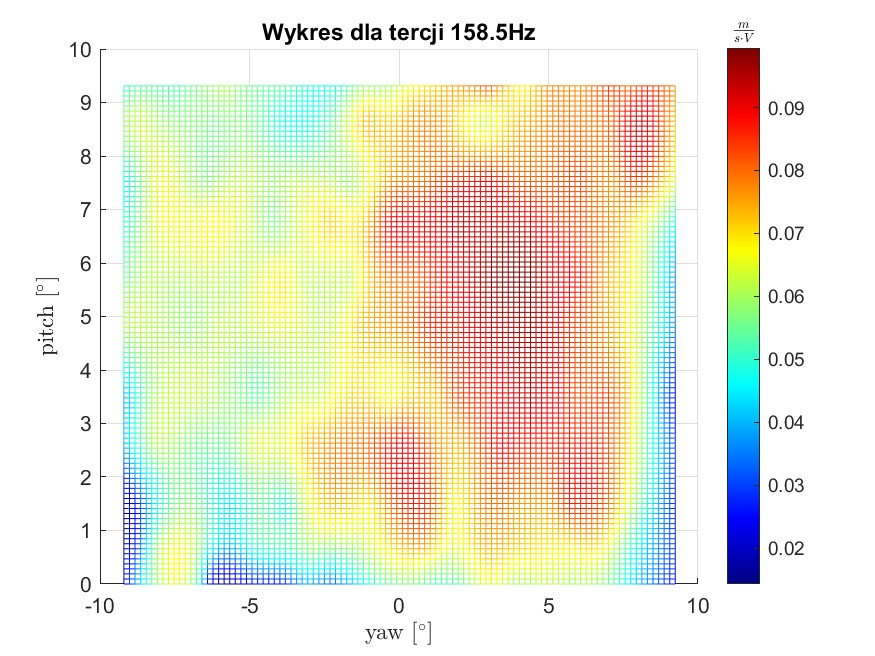
\includegraphics[width=0.8\textwidth]{img/9_GraphThird.jpg}
\caption{Rozkład drgań dla tercji $158.5Hz$.}
\label{img:9_GraphThird}
\end{figure}

Podobne zachowanie można zaobserwować poprzez wszystkie tercje o wyższych częstotliwościach środkowych. Wszędzie drgania są wyraźnie mocniejsze po prawej stronie płyty. Także zależnie od częstotliwości, albo cała prawa strona drga jednolicie, albo można nakreślić wyraźne punkty - strzałki drgań - w których drgania są zdecydowanie mocniejsze. Pomimo że następuje też statyczny spadek amplitudy drgań, i dla częstotliwości $4kHz$ drgania są już na poziomie zaledwie $10^{-2}$-$10^{-3}$, to należy pamiętać wykres \ref{img:background_noise_graph}, gdzie dla tych częstotliwości poziom szumów tła spadł do poziomu $5 \cdot 10^{-4}$, co oznacza, że nawet najsłabsze drgania dla tych częstotliwości, przy włączonym głośniku są nadal 20-krotnie wyższe niż przy głośniku wyłączonym. Rozkład drgań dla opisywanej częstotliwości opisuje wykres \ref{img:23_GraphThird}.

\begin{figure}[h!] 
\centering 
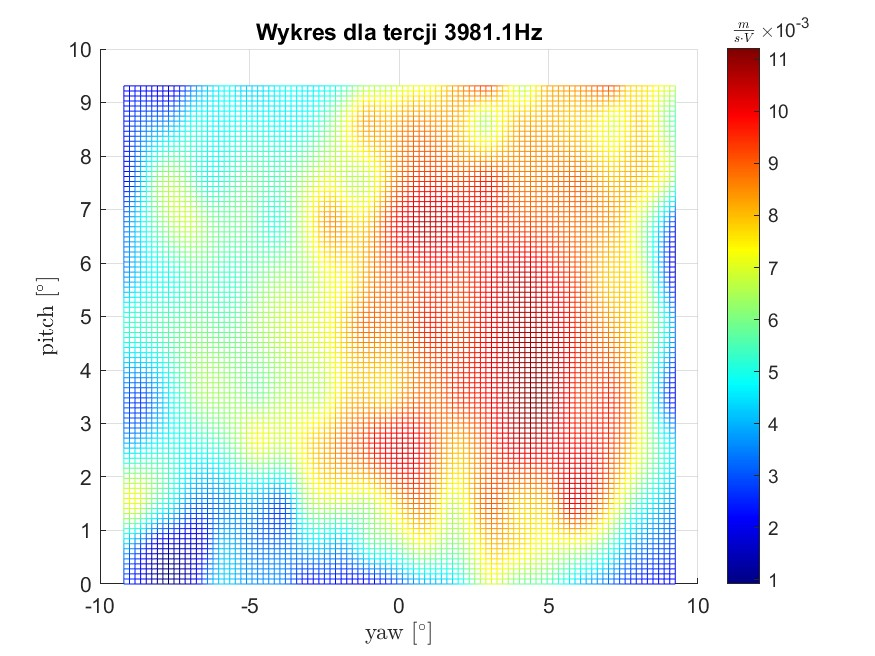
\includegraphics[width=0.8\textwidth]{img/23_GraphThird.jpg}
\caption{Rozkład drgań dla tercji $4kHz$.}
\label{img:23_GraphThird}
\end{figure}